\documentclass[conference]{IEEEtran}

\usepackage{cite}
\usepackage{amsmath,amssymb,amsfonts}
\usepackage{graphicx}
\usepackage{booktabs}
\usepackage{textcomp}
\usepackage{xcolor}

\def\BibTeX{{\rm B\kern-.05em{\sc i\kern-.025em b}\kern-.08em
    T\kern-.1667em\lower.7ex\hbox{E}\kern-.125emX}}

\begin{document}

\title{GAD-MambaUNet: Direction-Group Mamba with Gradient-Adaptive DINOv3 Distillation for Lightweight Medical Image Segmentation}

\author{\IEEEauthorblockN{Anonymous Author(s)}
\IEEEauthorblockA{Anonymous Affiliation\\
Anonymous City, Country\\
anonymous@example.com}}

\maketitle

% \begin{abstract}
% Lightweight medical image segmentation requires accurate delineation of local lesion boundaries under strict computational constraints. Lightweight convolutional networks efficiently preserve local details, but their limited receptive fields make long-range dependency modeling difficult. Although Transformer-based methods improve global modeling, they often introduce substantial computational overhead. Visual state-space models, represented by Mamba, provide an alternative with linear-complexity global modeling, while grouped Mamba further reduces computational cost by partitioning feature channels into multiple groups. However, conventional grouped multi-directional scans process different channel groups and scanning directions independently before fusion, limiting the exchange of complementary contextual information. We propose GAD-MambaUNet, an asymmetric local--global segmentation network with Direction-Group Graph Selective Scan (DG-GSS) blocks. DG-GSS explicitly models direction--group feature responses as graph nodes and performs structured message passing before multi-directional fusion, thereby integrating complementary spatial context across scanning directions and feature subspaces. Furthermore, we introduce a frozen pretrained DINOv3 model as a semantic teacher and transfer its rich semantic priors to the compact student through Gradient-Adaptive Distillation. Extensive experiments on the BUSI breast ultrasound, ISIC2018 dermoscopy, CVC-ClinicDB, and CVC-ColonDB colonoscopy datasets demonstrate that the proposed method achieves an average Dice score of \textit{XX.XX}\% with only \textit{XX.XX}M parameters and \textit{XX.XX}G FLOPs.
% \end{abstract}

\begin{abstract}
Lightweight medical image segmentation requires accurate delineation of subtle lesion boundaries under strict computational constraints. Convolutional encoder--decoder networks are effective in preserving local details, but their limited receptive fields make it difficult to capture long-range dependencies. Transformer-based methods improve global context modeling, yet often introduce considerable computational and memory overhead. Visual state-space models, such as Mamba, provide an efficient alternative for global modeling with linear complexity, and grouped Mamba further reduces computation by partitioning feature channels into multiple groups. However, existing grouped multi-directional scanning strategies usually process different channel groups and scanning directions independently before fusion, which limits the exchange of complementary contextual information.
To address this limitation, we propose GAD-MambaUNet, an asymmetric local--global segmentation network for lightweight medical image segmentation. The proposed network uses lightweight convolutional blocks in shallow stages to preserve fine boundary details and introduces Direction-Group Graph Selective Scan (DG-GSS) blocks in deeper stages for efficient contextual modeling. In each DG-GSS block, direction--group feature responses are represented as graph nodes, and structured message passing is performed before multi-directional fusion, enabling interaction across scanning directions and feature subspaces. To further enhance semantic representation without increasing inference cost, a frozen pretrained DINOv3 model is used only during training as a semantic teacher, and its semantic priors are transferred to the compact student through Gradient-Adaptive Distillation. Experiments on multiple public medical image segmentation datasets demonstrate that GAD-MambaUNet achieves an average Dice score of \textit{XX.XX}% with only \textit{XX.XX}M parameters and \textit{XX.XX}G FLOPs, showing a favorable balance between segmentation accuracy and model efficiency.
\end{abstract}

\begin{IEEEkeywords}
medical image segmentation, lightweight networks, state-space models, DINOv3, knowledge distillation
\end{IEEEkeywords}

\iffalse
\section{Introduction}

Accurate medical image segmentation is essential for computer-aided diagnosis, treatment planning, and quantitative disease assessment. In practical settings, a useful segmentation model must delineate subtle lesions and tumors while remaining small enough for point-of-care, mobile, or edge deployment. This objective is difficult because medical targets often occupy only a small image region, exhibit weak or irregular boundaries, and appear under modality-specific artifacts. Dermoscopy, ultrasound, and colonoscopy all present different visual degradations, but they share the same core requirement: the model must preserve local boundary evidence while exploiting broader context to resolve ambiguous foreground-background appearance.

U-Net~\cite{ronneberger2015unet} and its variants established the encoder--decoder paradigm for medical segmentation by combining deep semantic features with high-resolution skip connections. Polyp-specific and attention-based networks such as PraNet~\cite{fan2020pranet} and UACANet~\cite{kim2021uacanet} improve boundary refinement and ambiguity handling, while Transformer-based models such as TransUNet~\cite{chen2021transunet} introduce stronger global context. However, many of these methods increase parameters, memory, or computation, which is undesirable for lightweight clinical deployment.

Recent lightweight models reduce this burden through depth-wise convolutions, compact channel schedules, grouped attention, and inexpensive token mixing. UNeXt~\cite{valanarasu2022unext}, CMUNeXt~\cite{tang2024cmunext}, EGE-UNet~\cite{ruan2023egeunet}, EMCAD~\cite{rahman2024emcad}, and MK-UNet~\cite{rahman2025mkunet} demonstrate that careful operator design can achieve strong segmentation performance with reduced complexity. A common strength of these models is their local inductive bias: they are effective at capturing texture, boundary, and multi-scale appearance cues. The remaining challenge is to add global contextual reasoning without losing the computational and boundary-preserving advantages that make lightweight models attractive.

Selective state-space models provide a promising alternative for efficient global modeling. Mamba~\cite{gu2023mamba} introduces input-dependent sequence modeling with linear complexity, and VMamba~\cite{liu2024vmamba} extends selective scanning to two-dimensional vision features. UltraLight VM-UNet~\cite{wu2024ultralight} further shows the potential of parallel Vision Mamba branches for lightweight medical segmentation. However, simply splitting channels into groups and scanning in multiple directions can fragment complementary responses before fusion if direction and group interactions are not explicitly modeled. This is undesirable for medical images, where a weak boundary may need to be interpreted using both local texture and distant contextual cues.

Large self-supervised vision models provide another way to improve semantic consistency. DINOv3~\cite{simeoni2025dinov3} produces dense representations that can guide compact students. Yet a fixed knowledge distillation coefficient~\cite{hinton2015distilling} is brittle for a small segmentation model: too much teacher pressure early may interfere with mask learning, while too little teacher guidance later may fail to transfer global semantics. This motivates a training strategy that adjusts the teacher contribution according to the student optimization state.

We propose \emph{GAD-MambaUNet}, a lightweight segmentation framework organized around local-detail preservation, efficient global interaction, and stable semantic transfer. First, the network keeps multi-kernel convolutional processing at high-resolution stages and uses grouped state-space blocks only in deeper stages, where global context is cheaper to model. Second, we propose Direction-Group Graph Selective Scan (DG-GSS), which represents each scanning-direction and channel-group pair as a graph node and learns content-dependent interactions before directional fusion. Third, we distill dense DINOv3 features at the deepest decoder stage and regulate the distillation strength with Gradient-Adaptive Distillation (GAD), which monitors the gradient share of the aligned decoder block.

Our contributions are summarized as follows:
\begin{itemize}
    \item We develop a lightweight architecture for multi-source binary medical segmentation that targets boundary-sensitive lesions and tumors across different imaging modalities.
    \item We introduce an asymmetric local--global design that preserves high-resolution multi-kernel convolution while using grouped visual state-space modeling at deep semantic stages.
    \item We propose DG-GSS to explicitly exchange information among scanning directions and channel groups before state-space directional fusion.
    \item We introduce Gradient-Adaptive DINOv3 Distillation, which transfers foundation-model semantics during training without adding teacher-side inference cost.
\end{itemize}

\section{Related Work}

\subsection{Medical Image Segmentation Networks}

Binary medical image segmentation covers diverse imaging modalities and clinical targets. Dermoscopic skin lesion segmentation, breast ultrasound tumor segmentation, and colonoscopic polyp segmentation all require accurate foreground delineation, but they expose different visual challenges such as irregular lesion shapes, speckle noise, low-contrast tumor boundaries, mucosal texture similarity, illumination artifacts, and cross-source variation. Public benchmarks including ISIC2018~\cite{codella2019skin}, BUSI~\cite{al2020dataset}, CVC-ClinicDB~\cite{bernal2015clinicdb}, and CVC-ColonDB~\cite{vazquez2017benchmark} are therefore useful for evaluating whether a lightweight model is merely specialized or broadly robust.

U-Net~\cite{ronneberger2015unet} remains a foundational architecture because its skip connections combine local detail with semantic context. Later CNN and attention variants improve this design through nested skips, attention gates, reverse attention, uncertainty modeling, and multi-scale decoding. PraNet~\cite{fan2020pranet} is a representative polyp segmentation network using parallel partial decoding and reverse attention, while UACANet~\cite{kim2021uacanet} uses uncertainty-augmented context attention. TransUNet~\cite{chen2021transunet} and related Transformer models strengthen global modeling but often depend on heavier token interaction or pretrained backbones.

\subsection{Lightweight Segmentation}

Lightweight medical segmentation models aim to balance segmentation accuracy with small parameter count and low computation. UNeXt~\cite{valanarasu2022unext} combines convolutional encoders with shifted MLP blocks, CMUNeXt~\cite{tang2024cmunext} uses large kernels and skip fusion, EGE-UNet~\cite{ruan2023egeunet} develops group-enhanced attention, and EMCAD~\cite{rahman2024emcad} introduces an efficient multi-scale convolutional attention decoder.

Among these methods, MK-UNet~\cite{rahman2025mkunet} is a representative multi-kernel lightweight design. Its Multi-Kernel Inverted Residual (MKIR) block applies parallel depth-wise kernels, channel shuffle, and point-wise projection to capture local patterns at several receptive-field scales with a compact footprint. Its decoder further uses channel attention, spatial attention, and grouped attention gates. These components are well suited to boundary-sensitive medical segmentation, so our design preserves the same local modeling spirit. The difference is that we do not rely on local operators alone: deep low-resolution stages are assigned to grouped state-space modeling and training-time semantic distillation.

\subsection{Visual State-Space Models}

State-space models have recently become an efficient alternative to self-attention for long-range dependency modeling. Mamba~\cite{gu2023mamba} uses selective input-dependent state transitions with linear complexity. VMamba~\cite{liu2024vmamba} adapts selective scanning to visual features through multiple two-dimensional traversal directions. UltraLight VM-UNet~\cite{wu2024ultralight} shows that channel-wise parallel Vision Mamba branches can substantially reduce model size for medical segmentation.

However, efficient grouping introduces a representation-isolation problem. Directional scans encode complementary spatial contexts, and channel groups encode different feature subspaces, but conventional fusion often merges them without adaptive interaction. Our DG-GSS module explicitly constructs a factorized graph over direction--group nodes. Nodes communicate when they share either a scanning direction or a channel-group identity, enabling structured information exchange while preserving the efficiency of grouped selective scans.

\subsection{Foundation-Model Distillation}

Knowledge distillation transfers information from a high-capacity teacher to a compact student~\cite{hinton2015distilling}. Dense feature distillation is especially useful for segmentation because it provides spatial supervision beyond output logits. DINOv3~\cite{simeoni2025dinov3} offers strong dense self-supervised representations and can serve as a training-time teacher for heterogeneous medical images.

Most distillation methods use a fixed loss coefficient. In lightweight medical segmentation, this can be suboptimal because the student first needs to learn task-specific masks and only later can reliably absorb stronger semantic guidance. We therefore use a staged schedule: segmentation-only burn-in, linear distillation warm-up, and gradient-adaptive coefficient control. The teacher is removed at inference, keeping deployment cost determined solely by the compact student.


\begin{figure*}[t]
    \centering
    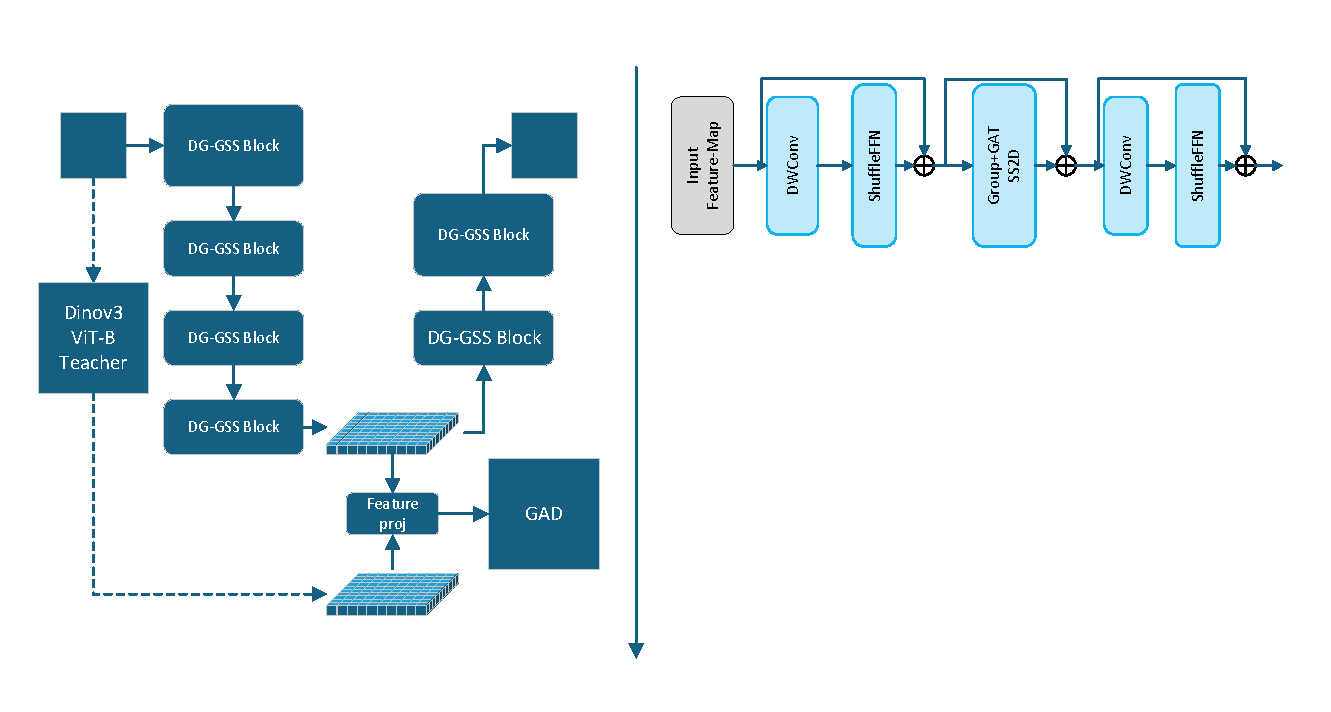
\includegraphics[width=\textwidth]{all-network.pdf}
    \caption{Overall architecture of GAD-MambaUNet. The student uses multi-kernel convolutional processing at high-resolution stages and introduces DG-GSS blocks at deep semantic stages. During training, a frozen DINOv3 teacher provides dense feature supervision at the first decoder block, while GAD regulates the distillation coefficient according to the aligned block's gradient share. The teacher and projection head are removed during inference.}
    \label{fig:overall-network}
\end{figure*}


\section{Methodology}



\subsection{Overview}

As illustrated in Fig.~\ref{fig:overall-network}, given an input medical image $\mathbf{x}\in\mathbb{R}^{3\times H\times W}$, the student predicts a binary segmentation logit map $\mathbf{z}\in\mathbb{R}^{1\times H\times W}$. The base configuration uses a compact five-level U-shaped hierarchy with channel dimensions $[16,32,64,96,160]$. The first three encoder stages and the last three decoder stages use Multi-Kernel Inverted Residual blocks to retain local texture and boundary cues. The two deepest encoder stages and the first two decoder stages use grouped state-space blocks for efficient context modeling. Depth-wise separable downsampling and point-wise projection handle resolution and channel transitions outside the state-space blocks, and grouped attention gates refine skip fusion.

Training combines a structure-aware segmentation objective with dense feature alignment from a frozen DINOv3 teacher. The aligned student feature is taken after the first decoder block and before upsampling, at approximately $H/32\times W/32$. This point is semantically strong, computationally cheap, and directly associated with the deep decoder block monitored by GAD.

\subsection{Asymmetric Local--Global Student}

For high-resolution stages, we use a multi-kernel inverted residual block. A block expands channels with a $1\times1$ convolution, applies parallel depth-wise convolutions with kernel sizes $\{1,3,5\}$, sums their outputs, shuffles channels, and projects them back to the target dimension. The multi-kernel design captures small lesion edges, ultrasound texture variations, and polyp boundary patterns at low computational cost.

At low-resolution stages, each Grouped Mamba block applies depth-wise local mixing, a grouped feed-forward network, the DG-GSS operator, and a second local feed-forward refinement. Residual paths surround these components. Channel expansion and reduction are kept outside the state-space operator and handled by downsampling or upsampling modules, which keeps the selective scan dimension fixed inside each block.

Before skip fusion, a grouped attention gate modulates encoder features using the current decoder feature. Let $\mathbf{g}$ be an upsampled decoder feature and $\mathbf{s}$ be the same-resolution encoder feature. The gate computes
\begin{equation}
\boldsymbol{\alpha}=\sigma\!\left(\psi\left(\phi(W_g\mathbf{g}+W_s\mathbf{s})\right)\right),
\end{equation}
where $W_g$ and $W_s$ are grouped convolutions, $\phi$ is a nonlinear activation, and $\psi$ maps the response to a spatial attention map. The gated skip feature $\hat{\mathbf{s}}=\boldsymbol{\alpha}\odot\mathbf{s}$ is added to the decoder feature.

\subsection{Direction-Group Graph Selective Scan}

Let $\mathbf{X}\in\mathbb{R}^{B\times D\times h\times w}$ denote a deep feature map. DG-GSS uses $K=4$ scanning directions and partitions the $D$ channels into $M$ groups of width $d=D/M$. Cross scanning produces
\begin{equation}
\mathbf{X}_{\mathrm{scan}}\in\mathbb{R}^{B\times K\times M\times d\times L},
\qquad L=hw.
\end{equation}
Each direction--group pair generates its own selective-scan parameters $(\Delta,\mathbf{B},\mathbf{C})$. After selective scanning, the outputs are spatially aligned to the original image coordinates and reshaped as
\begin{equation}
\mathbf{Y}\in\mathbb{R}^{B\times K\times M\times d\times h\times w}.
\end{equation}

Each pair $(k,m)$ is treated as a graph node. A node descriptor is obtained by global average pooling:
\begin{equation}
\mathbf{r}_{k,m}=\frac{1}{hw}\sum_{u,v}\mathbf{Y}_{k,m,:,u,v}.
\end{equation}
After layer normalization and projection, additive graph-attention logits are computed as
\begin{equation}
e_{ij}=\operatorname{LeakyReLU}\left(\mathbf{a}_{s}^{\top}\mathbf{h}_i+
\mathbf{a}_{t}^{\top}\mathbf{h}_j\right).
\end{equation}
The factorized graph connects nodes that share either a scanning direction or a channel-group identity. With masked softmax coefficients $a_{ij}$ and a shared $1\times1$ value projection $V(\cdot)$, graph propagation is
\begin{equation}
\widetilde{\mathbf{Y}}_i=\mathbf{Y}_i+\gamma\sum_{j\in\mathcal{N}(i)}a_{ij}V(\mathbf{Y}_j),
\end{equation}
where $\gamma$ is learnable and initialized to zero. The final output concatenates channel groups and sums the aligned directional responses.

\subsection{DINOv3 Feature Distillation}

A frozen DINOv3 ViT-B/16 teacher provides dense semantic features during training. The student feature $\mathbf{F}_s$ from the first decoder block is projected to the teacher dimension by a $1\times1$ convolution and batch normalization. The teacher feature $\mathbf{F}_t$ is resized if necessary. Both features are flattened into spatial tokens and $\ell_2$ normalized. The distillation loss is
\begin{equation}
\mathcal{L}_{\mathrm{dist}}=
\frac{1}{N}\sum_{n=1}^{N}\left[1-
\frac{\mathbf{f}_{s,n}^{\top}\mathbf{f}_{t,n}}
{\|\mathbf{f}_{s,n}\|_2\|\mathbf{f}_{t,n}\|_2}\right].
\end{equation}
The segmentation term follows a structure-aware objective commonly used in boundary-sensitive medical segmentation~\cite{fan2020pranet}:
\begin{equation}
\mathcal{L}=\mathcal{L}_{\mathrm{seg}}+\lambda_e\mathcal{L}_{\mathrm{dist}},
\qquad
\mathcal{L}_{\mathrm{seg}}=\mathcal{L}_{\mathrm{wbce}}+\mathcal{L}_{\mathrm{wiou}}.
\end{equation}

\subsection{Gradient-Adaptive Distillation}

After backpropagation and before gradient clipping, GAD computes the gradient share of the aligned decoder stage:
\begin{equation}
q_e=100\times
\frac{\sum_{\theta_i\in\Theta_a}\|\nabla_{\theta_i}\mathcal{L}\|_1}
{\sum_{\theta_j\in\Theta}\|\nabla_{\theta_j}\mathcal{L}\|_1}.
\end{equation}
Here, $\Theta_a$ denotes parameters of the aligned decoder block and $\Theta$ denotes all trainable student parameters. If $q_e$ lies outside the desired interval $[\rho-\delta,\rho+\delta]$, a target share $q^{*}$ is selected at the opposite interval boundary and an odds-ratio update is computed:
\begin{equation}
r_e=\frac{p^{*}(1-p_e)}{p_e(1-p^{*})},
\quad p_e=q_e/100,\quad p^{*}=q^{*}/100.
\end{equation}
The next base distillation coefficient is
\begin{equation}
\lambda_{e+1}=\operatorname{clip}\left(
\lambda_e\operatorname{clip}(r_e,r_{\min},r_{\max}),
\lambda_{\min},\lambda_{\max}\right).
\end{equation}
Training starts with segmentation-only burn-in, then linearly warms up distillation, and finally activates GAD. During inference, DINOv3 and the projection head are discarded.

\fi

% \section{Introduction}

% Accurate medical image segmentation is fundamental to computer-aided diagnosis, treatment planning, and quantitative disease assessment. Given a medical image, the goal is to delineate clinically relevant structures at the pixel level while preserving their boundaries and spatial extent. This task is challenging because medical targets can be small, irregular, weakly contrasted, or visually similar to surrounding tissue. A useful segmentation model must therefore combine fine-grained local evidence, which is needed for boundary recovery, with sufficient contextual information to distinguish ambiguous foreground and background regions.

% U-Net~\cite{ronneberger2015unet} established the dominant encoder--decoder paradigm for medical image segmentation. Its contracting path extracts increasingly abstract semantic representations, while skip connections transfer high-resolution encoder features to the decoder for spatially precise reconstruction. Building on this design, numerous CNN-based methods have improved feature fusion, attention, boundary refinement, and multi-scale decoding. For example, PraNet~\cite{fan2020pranet} uses parallel partial decoding and reverse attention for polyp segmentation, whereas UACANet~\cite{kim2021uacanet} introduces uncertainty-aware context attention. These methods demonstrate the importance of combining semantic understanding with accurate localization.

% Despite their success, convolutional networks have an intrinsic limitation: their local receptive fields do not directly capture long-range dependencies. This limitation becomes evident when boundary interpretation requires global lesion shape, long-range boundary continuity, or contextual contrast between foreground targets and surrounding tissues. Transformer-based networks, such as TransUNet~\cite{chen2021transunet}, address this issue by introducing self-attention for global feature interaction. However, global attention and large pretrained backbones can substantially increase parameter count, memory usage, and computational cost. Thus, stronger contextual modeling does not automatically translate into a practical solution when inference resources are limited.

% \begin{figure*}[!t]
%     \centering
%     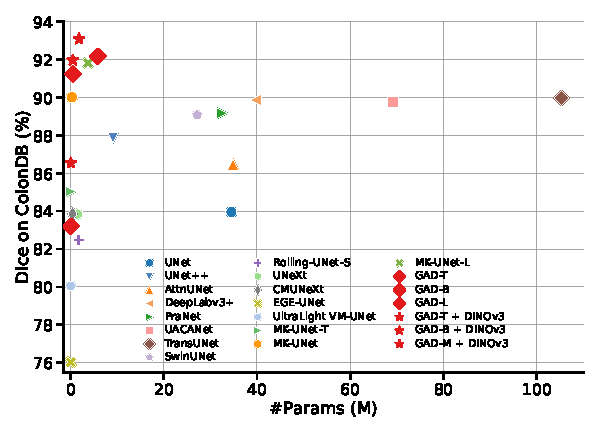
\includegraphics[width=0.49\textwidth]{figures/avg_dice_params.pdf}\hfill
%     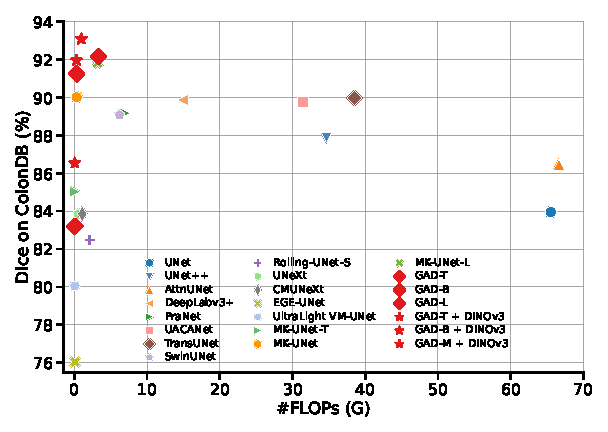
\includegraphics[width=0.49\textwidth]{figures/avg_dice_flops.pdf}
%     \caption{ColonDB accuracy--efficiency comparison. Left: Dice versus student-side parameters. Right: Dice versus FLOPs. Reference values are from the MK-UNet comparison protocol, whose FLOPs are reported at $256\times256$ input resolution; they are used here for a uniform relative comparison. GAD-MambaUNet uses Tiny, Base, and Large variants, while the DINOv3 setting uses Tiny, Base, and Medium variants. DINOv3 is a training-only teacher and is excluded from deployment cost.}
%     \label{fig:colondb-efficiency}
% \end{figure*}

% As medical imaging solutions increasingly move from laboratory-centered analysis to point-of-care applications, segmentation accuracy is no longer the only design objective. Parameter count, computational complexity, memory footprint, and inference efficiency also determine whether a model can be used in realistic clinical or edge-device settings. This transition has motivated lightweight medical segmentation networks based on depth-wise convolution, compact channel schedules, grouped operators, and efficient token mixing. UNeXt~\cite{valanarasu2022unext}, CMUNeXt~\cite{tang2024cmunext}, EGE-UNet~\cite{ruan2023egeunet}, and EMCAD~\cite{rahman2024emcad} are representative examples. In particular, MK-UNet~\cite{rahman2025mkunet} uses multi-kernel depth-wise convolution and lightweight decoder attention to retain local multi-scale modeling at a compact cost. Nevertheless, lightweight CNN-dominated backbones can still lack the global evidence needed when boundaries are incomplete or distant regions share similar texture.

% Visual state-space models provide a promising route to efficient global modeling. Mamba~\cite{gu2023mamba} models input-dependent sequences with linear complexity, and VMamba~\cite{liu2024vmamba} extends selective scanning to two-dimensional visual features. VM-UNet~\cite{ruan2024vmunet} integrates visual state-space blocks into a U-shaped architecture for medical image segmentation. To further reduce the cost of Vision Mamba, UltraLight VM-UNet~\cite{wu2024ultralight} partitions deep features into multiple parallel channel groups and processes them using parallel Vision Mamba branches. This design reduces the parameter and computational cost of global modeling. However, partitioning features into groups also creates a representation-isolation issue. In conventional grouped multi-directional selective scanning, each direction--group branch is processed independently and the responses are merged only after selective scanning. Consequently, complementary context from different traversal directions and channel groups cannot influence one another before fusion. This limitation motivates our DG-GSS, which enables structured direction--group interaction before multi-directional fusion.

% To address these issues, we propose \emph{GAD-MambaUNet}, an asymmetric local--global U-shaped network for lightweight medical image segmentation. The architecture preserves multi-kernel convolution at high-resolution stages, where local texture extraction and boundary reconstruction are most important, and introduces grouped state-space blocks at deep low-resolution stages, where global reasoning is more economical. Within each state-space block, we propose Direction-Group Graph Selective Scan (DG-GSS). DG-GSS represents each scan-direction and channel-group response as a graph node, then enables structured information exchange among nodes sharing the same direction or the same channel-group identity before multi-directional fusion. In addition, a frozen DINOv3 teacher~\cite{simeoni2025dinov3} provides dense semantic supervision during training. Drawing on gradient-guided semantic modulation for real-time detection~\cite{liao2025rtdetrv4}, Gradient-Adaptive Distillation (GAD) regulates the distillation coefficient from the gradient share of the aligned decoder block; the teacher and projection head are discarded during inference. To evaluate the proposed method, we conduct experiments on PH$^2$, ISIC2018, CVC-ClinicDB, and CVC-ColonDB. Fig.~\ref{fig:colondb-efficiency} illustrates the available ColonDB accuracy--efficiency comparison.

% The contributions of this work are summarized as follows:
% \begin{itemize}
%     \item We develop an asymmetric lightweight U-shaped architecture that combines high-resolution multi-kernel local modeling with deep grouped state-space modeling for efficient context aggregation.
%     \item We propose DG-GSS, which explicitly exchanges information among direction--group responses before multi-directional fusion through a factorized graph.
%     \item We introduce training-time DINOv3 feature supervision with GAD, which regulates distillation using the gradient share of the aligned decoder block and adds no teacher-side inference cost.
% \end{itemize}





% \section{Introduction}

% Accurate medical image segmentation is fundamental to computer-aided diagnosis, treatment planning, and quantitative disease assessment. Given a medical image, the goal is to delineate clinically relevant structures at the pixel level while preserving their boundaries and spatial extent. This task is challenging because medical targets can be small, irregular, weakly contrasted, or visually similar to surrounding tissue. A useful segmentation model must therefore combine fine-grained local evidence, which is needed for boundary recovery, with sufficient contextual information to distinguish ambiguous foreground and background regions.

% U-Net~\cite{ronneberger2015unet} established the dominant encoder--decoder paradigm for medical image segmentation. Its contracting path extracts increasingly abstract semantic representations, while skip connections transfer high-resolution encoder features to the decoder for spatially precise reconstruction. Building on this design, numerous CNN-based methods have improved feature fusion, attention, boundary refinement, and multi-scale decoding. For example, PraNet~\cite{fan2020pranet} uses parallel partial decoding and reverse attention for polyp segmentation, whereas UACANet~\cite{kim2021uacanet} introduces uncertainty-aware context attention. These methods demonstrate the importance of combining semantic understanding with accurate localization.

% Despite their success, convolutional networks have an intrinsic limitation: their local receptive fields do not directly capture long-range dependencies. This limitation becomes important when the correct interpretation of a boundary depends on distant structures or broader anatomical context. Transformer-based networks, such as TransUNet~\cite{chen2021transunet}, address this issue by introducing self-attention for global feature interaction. However, global attention and large pretrained backbones can substantially increase parameter count, memory usage, and computational cost. Thus, stronger contextual modeling does not automatically translate into a practical solution when inference resources are limited.

% \begin{figure*}[!t]
% \centering
% 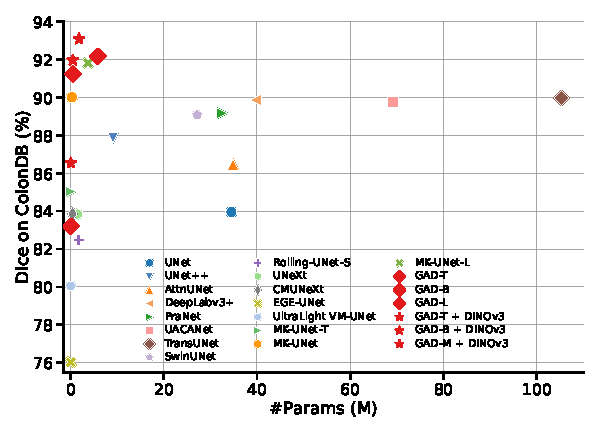
\includegraphics[width=0.49\textwidth]{figures/avg_dice_params.pdf}\hfill
% 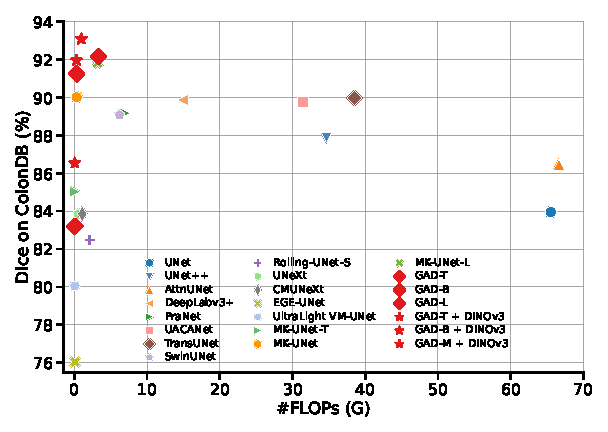
\includegraphics[width=0.49\textwidth]{figures/avg_dice_flops.pdf}
% \caption{Accuracy--efficiency comparison across PH$^2$, ISIC2018, CVC-ClinicDB, and CVC-ColonDB. The vertical axis reports the macro-average Dice score over the four datasets, while the horizontal axes show student-side parameters and FLOPs. The DINOv3 teacher is used only during training and is excluded from deployment cost.}
% \label{fig:efficiency-comparison}
% \end{figure*}

% As medical imaging solutions increasingly move from laboratory-centered analysis to point-of-care applications, segmentation accuracy is no longer the only design objective. Parameter count, computational complexity, memory footprint, and inference efficiency also determine whether a model can be deployed in realistic clinical or edge-device settings. Following this accuracy--efficiency perspective, Fig.~\ref{fig:efficiency-comparison} summarizes the trade-off between average segmentation performance and deployment cost across the evaluated medical image segmentation benchmarks.

% This transition has motivated lightweight medical segmentation networks based on depth-wise convolution, compact channel schedules, grouped operators, and efficient token mixing. UNeXt~\cite{valanarasu2022unext}, CMUNeXt~\cite{tang2024cmunext}, EGE-UNet~\cite{ruan2023egeunet}, and EMCAD~\cite{rahman2024emcad} are representative examples. In particular, MK-UNet~\cite{rahman2025mkunet} uses multi-kernel depth-wise convolution and lightweight decoder attention to retain local multi-scale modeling at a compact cost. Nevertheless, lightweight CNN-dominated backbones can still lack the global evidence needed when boundaries are incomplete, lesion regions are ambiguous, or distant anatomical structures share similar textures.

% Visual state-space models provide a promising route to efficient global modeling. Mamba~\cite{gu2023mamba} models input-dependent sequences with linear complexity, and VMamba~\cite{liu2024vmamba} extends selective scanning to two-dimensional visual features. VM-UNet~\cite{ruan2024vmunet} integrates visual state-space blocks into a U-shaped architecture for medical image segmentation. Compared with global self-attention, selective scanning offers a more efficient mechanism for long-range dependency modeling, making it attractive for lightweight segmentation networks.

% To further reduce the cost of Vision Mamba, UltraLight VM-UNet~\cite{wu2024ultralight} partitions deep features into multiple parallel channel groups and processes them using parallel Vision Mamba branches. This design reduces the parameter and computational cost of global modeling. However, partitioning features into groups also creates a representation-isolation issue. In conventional grouped multi-directional selective scanning, each direction--group branch is processed independently, and the responses are merged only after selective scanning. Consequently, complementary context from different traversal directions and channel groups cannot influence one another before fusion. This limitation motivates a more structured mechanism for direction--group interaction.

% To address these issues, we propose \emph{GAD-MambaUNet}, an asymmetric local--global U-shaped network for lightweight medical image segmentation. The architecture preserves multi-kernel convolution at high-resolution stages, where local texture extraction and boundary reconstruction are most important, and introduces grouped state-space blocks at deep low-resolution stages, where global reasoning is more economical. Within each state-space block, we propose Direction-Group Graph Selective Scan (DG-GSS), which represents each scan-direction and channel-group response as a graph node and enables structured information exchange among nodes sharing the same direction or the same channel-group identity before multi-directional fusion.

% Beyond architecture design, compact segmentation models trained on limited medical datasets may still suffer from insufficient semantic abstraction. Inspired by the DINOv3-based gradient-adaptive distillation strategy in RT-DETRv4~\cite{liao2025rtdetrv4}, we adapt training-time foundation-model supervision to lightweight medical image segmentation. Specifically, a frozen DINOv3 teacher~\cite{simeoni2025dinov3} provides dense semantic supervision for the aligned decoder feature, while Gradient-Adaptive Distillation (GAD) adjusts the distillation coefficient according to the gradient share of this decoder block. The teacher and projection head are discarded during inference, so the semantic supervision introduces no additional deployment cost.

% To evaluate the proposed method, we conduct experiments on PH$^2$, ISIC2018, CVC-ClinicDB, and CVC-ColonDB. The contributions of this work are summarized as follows:

% \begin{itemize}
% \item We develop an asymmetric local--global U-shaped architecture that preserves high-resolution multi-kernel convolution for boundary-sensitive local modeling and introduces grouped state-space modeling at deep semantic stages for efficient context aggregation.

% \item We propose DG-GSS, which explicitly exchanges information among direction--group responses through a factorized graph before multi-directional selective-scan fusion.

% \item We adapt RT-DETRv4-style DINOv3 feature supervision and gradient-adaptive distillation to lightweight medical image segmentation, aligning teacher features with a deep decoder block while adding no teacher-side inference cost.
% \end{itemize}







% \section{Introduction}

% Accurate medical image segmentation is fundamental to computer-aided diagnosis, treatment planning, and quantitative disease assessment. Given a medical image, the goal is to delineate clinically relevant structures at the pixel level while preserving their boundaries and spatial extent. This task remains challenging because medical targets are often small, irregular, weakly contrasted, and visually similar to surrounding tissues. Therefore, an effective segmentation model must simultaneously capture fine-grained local details for boundary recovery and sufficient contextual information for discriminating ambiguous foreground and background regions.

% U-Net~\cite{ronneberger2015unet} established the dominant encoder--decoder paradigm for medical image segmentation. Its contracting path extracts hierarchical semantic representations, while skip connections transfer high-resolution encoder features to the decoder for spatially precise reconstruction. Based on this paradigm, many CNN-based methods have improved medical image segmentation through multi-scale feature extraction, attention-based feature refinement, boundary-aware learning, and enhanced decoder design. For example, PraNet~\cite{fan2020pranet} employs parallel partial decoding and reverse attention for polyp segmentation, while UACANet~\cite{kim2021uacanet} introduces uncertainty-aware context attention to refine ambiguous regions. These methods demonstrate that local texture modeling and high-resolution feature reuse are crucial for accurate medical segmentation.

% However, convolutional networks are inherently limited by their local receptive fields. Although stacking convolutional layers can enlarge the effective receptive field, long-range dependencies are still captured indirectly and may be insufficient when the interpretation of a lesion boundary depends on distant anatomical context. Transformer-based methods, such as TransUNet~\cite{chen2021transunet}, introduce self-attention to model global feature interactions and have achieved promising performance in medical image segmentation. Nevertheless, global attention and large pretrained backbones often bring substantial computational cost, memory consumption, and parameter overhead. This makes it difficult to deploy such models in resource-constrained clinical or edge-device scenarios.

% As medical imaging solutions increasingly move from laboratory-centered analysis to point-of-care applications, segmentation accuracy is no longer the only design objective. Parameter count, computational complexity, memory footprint, and inference efficiency also determine whether a model can be practically deployed. As shown in Fig.~\ref{fig:efficiency-comparison}, the proposed method achieves a more favorable accuracy--efficiency balance than existing lightweight segmentation networks, obtaining higher average Dice scores under comparable or lower parameter and FLOP budgets. This observation motivates our design goal: improving global contextual modeling while preserving the compact deployment cost required for practical medical image segmentation.

% \begin{figure*}[!t]
% \centering
% 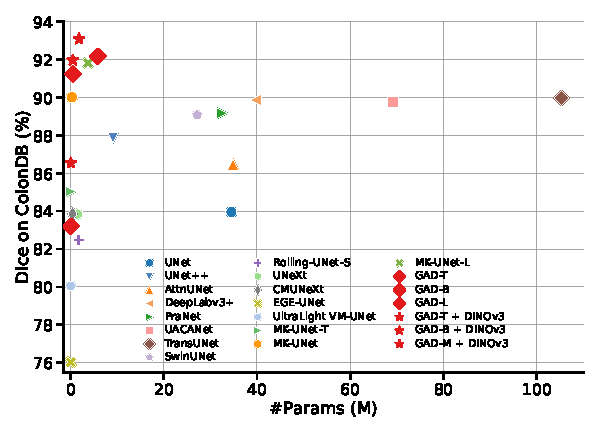
\includegraphics[width=0.49\textwidth]{figures/avg_dice_params.pdf}\hfill
% 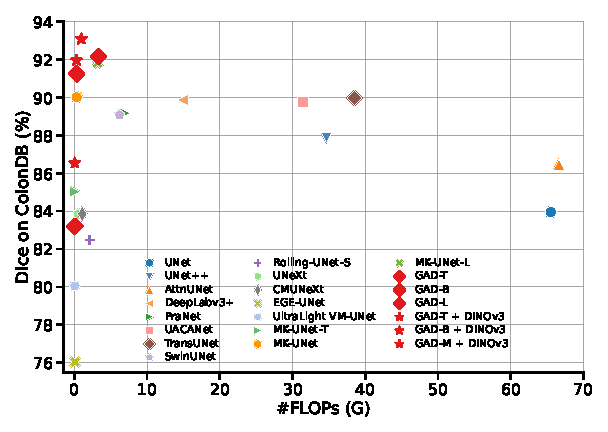
\includegraphics[width=0.49\textwidth]{figures/avg_dice_flops.pdf}
% \caption{Accuracy--efficiency comparison across PH$^2$, ISIC2018, CVC-ClinicDB, and CVC-ColonDB. The vertical axis reports the macro-average Dice score over the four datasets, while the horizontal axes show student-side parameters and FLOPs. Compared with existing lightweight segmentation networks, GAD-MambaUNet achieves a more favorable Pareto balance between segmentation accuracy and deployment cost. The DINOv3 teacher is used only during training and is excluded from deployment cost.}
% \label{fig:efficiency-comparison}
% \end{figure*}

% This accuracy--efficiency requirement has motivated lightweight medical segmentation networks based on depth-wise convolution, compact channel schedules, grouped operators, and efficient token mixing. UNeXt~\cite{valanarasu2022unext}, CMUNeXt~\cite{tang2024cmunext}, EGE-UNet~\cite{ruan2023egeunet}, and EMCAD~\cite{rahman2024emcad} are representative examples. In particular, MK-UNet~\cite{rahman2025mkunet} employs multi-kernel depth-wise convolution and lightweight decoder attention to preserve local multi-scale representation while maintaining a compact model size. Despite their efficiency, lightweight CNN-dominated backbones still have difficulty capturing global evidence when lesion regions are incomplete, boundaries are blurred, or distant anatomical structures share similar textures.

% Visual state-space models provide a promising alternative for efficient long-range dependency modeling. Mamba~\cite{gu2023mamba} introduces input-dependent selective state-space modeling with linear complexity, and VMamba~\cite{liu2024vmamba} extends selective scanning to two-dimensional visual features. VM-UNet~\cite{ruan2024vmunet} further integrates visual state-space blocks into a U-shaped architecture for medical image segmentation. Compared with global self-attention, selective scanning offers a more efficient way to model long-range dependencies, making it attractive for lightweight segmentation networks.

% To reduce the cost of Vision Mamba in medical segmentation, UltraLight VM-UNet~\cite{wu2024ultralight} partitions deep features into multiple channel groups and processes them using parallel Vision Mamba branches. This grouped design reduces parameters and computation while maintaining global modeling capability. However, channel grouping also introduces a representation-isolation issue. In conventional grouped multi-directional selective scanning, each direction--group branch is processed independently, and the responses are merged only after selective scanning. As a result, complementary information from different traversal directions and channel groups cannot interact before fusion. This limits the ability of grouped scanning to jointly exploit directional context and channel-subspace diversity.

% To address this limitation, we propose \emph{GAD-MambaUNet}, an asymmetric local--global U-shaped network for lightweight medical image segmentation. The architecture preserves multi-kernel convolution at high-resolution stages, where local texture extraction and boundary reconstruction are most important, and introduces grouped state-space blocks at deep low-resolution stages, where global reasoning can be performed more economically. Within each state-space block, we propose Direction-Group Graph Selective Scan (DG-GSS), which represents each scan-direction and channel-group response as a graph node. By performing structured message passing among nodes sharing the same direction or the same channel-group identity, DG-GSS enables explicit direction--group interaction before multi-directional fusion, thereby alleviating the representation-isolation issue in grouped selective scanning.

% Beyond architecture design, compact segmentation models trained on limited medical datasets may still suffer from insufficient semantic abstraction. Inspired by the DINOv3-based gradient-adaptive distillation strategy in RT-DETRv4~\cite{liao2025rtdetrv4}, we adapt training-time foundation-model supervision to lightweight medical image segmentation. Specifically, a frozen DINOv3 teacher~\cite{simeoni2025dinov3} provides dense semantic supervision for the aligned decoder feature, while Gradient-Adaptive Distillation (GAD) adjusts the distillation coefficient according to the gradient share of this decoder block. The teacher and projection head are discarded during inference, so the semantic supervision introduces no additional deployment cost.

% To evaluate the proposed method, we conduct experiments on PH$^2$, ISIC2018, CVC-ClinicDB, and CVC-ColonDB. The main contributions of this work are summarized as follows:

% \begin{itemize}
% \item We develop an asymmetric local--global U-shaped architecture that preserves high-resolution multi-kernel convolution for boundary-sensitive local modeling and introduces grouped state-space modeling at deep semantic stages for efficient context aggregation.

% \item We propose DG-GSS, which explicitly exchanges information among direction--group responses through a factorized graph before multi-directional selective-scan fusion, alleviating the representation-isolation issue in grouped selective scanning.

% \item We adapt RT-DETRv4-style DINOv3 feature supervision and gradient-adaptive distillation to lightweight medical image segmentation, aligning teacher features with a deep decoder block while adding no teacher-side inference cost.

% \item We conduct extensive experiments on PH$^2$, ISIC2018, CVC-ClinicDB, and CVC-ColonDB, showing that the proposed method achieves a superior accuracy--efficiency balance in terms of Dice score, parameters, and FLOPs compared with existing lightweight segmentation networks.
% \end{itemize}






\section{Introduction}

Accurate medical image segmentation is fundamental to computer-aided diagnosis, treatment planning, and quantitative disease assessment. Given a medical image, the goal is to delineate clinically relevant structures at the pixel level while preserving their boundaries and spatial extent. This task is challenging because medical targets are often small, irregular, weakly contrasted, or visually similar to surrounding tissue. A useful segmentation model must therefore combine fine-grained local evidence, which is essential for boundary recovery, with sufficient contextual information to distinguish ambiguous foreground and background regions.

U-Net~\cite{ronneberger2015unet} established the dominant encoder--decoder paradigm for medical image segmentation. Its contracting path extracts increasingly abstract semantic representations, while skip connections transfer high-resolution encoder features to the decoder for spatially precise reconstruction. Building on this design, numerous CNN-based methods have improved feature fusion, attention modeling, boundary refinement, and multi-scale decoding. For example, PraNet~\cite{fan2020pranet} uses parallel partial decoding and reverse attention for polyp segmentation, whereas UACANet~\cite{kim2021uacanet} introduces uncertainty-aware context attention. These methods demonstrate the importance of combining semantic understanding with accurate localization.

Despite their success, convolutional networks have an intrinsic limitation: their local receptive fields do not directly capture long-range dependencies. This limitation becomes evident when boundary interpretation requires global lesion shape, long-range boundary continuity, or contextual contrast between foreground targets and surrounding tissues. Transformer-based networks, such as TransUNet~\cite{chen2021transunet}, address this issue by introducing self-attention for global feature interaction. However, global attention and large pretrained backbones can substantially increase parameter count, memory usage, and computational cost. Thus, stronger contextual modeling does not automatically translate into a practical solution when inference resources are limited.

As medical imaging solutions increasingly move from laboratory-centered analysis to point-of-care applications, segmentation accuracy is no longer the only design objective. Parameter count, computational complexity, memory footprint, and inference efficiency also determine whether a model can be deployed in realistic clinical or edge-device settings. Therefore, an effective lightweight segmentation model should not only improve segmentation accuracy, but also maintain a favorable balance between accuracy and deployment cost.

\begin{figure*}[!t]
\centering
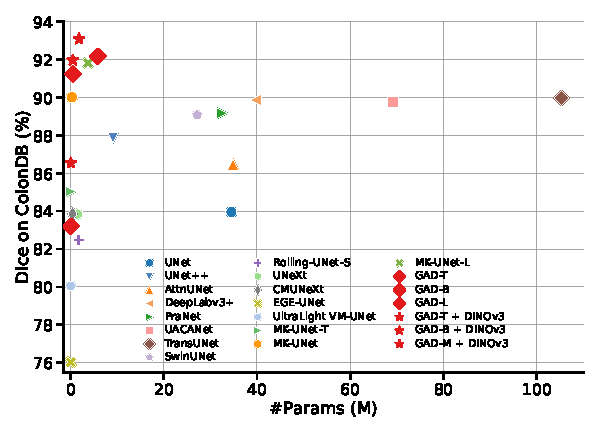
\includegraphics[width=0.49\textwidth]{figures/avg_dice_params.pdf}\hfill
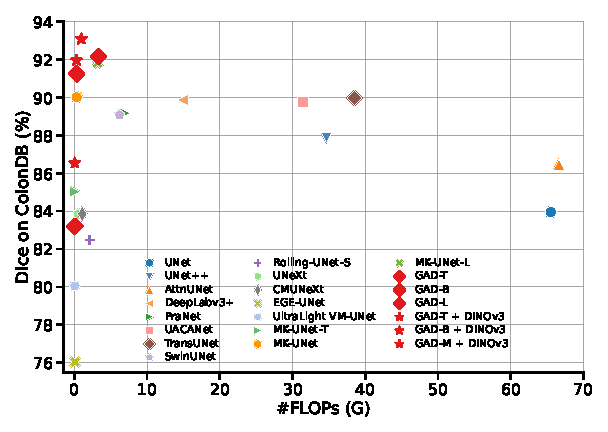
\includegraphics[width=0.49\textwidth]{figures/avg_dice_flops.pdf}
\caption{Accuracy--efficiency comparison across PH$^2$, ISIC2018, CVC-ClinicDB, and CVC-ColonDB. The vertical axis reports the macro-average Dice score over the four datasets, while the horizontal axes show student-side parameters and FLOPs. Compared with existing lightweight segmentation networks, GAD-MambaUNet achieves a more favorable balance between segmentation accuracy and deployment cost. The DINOv3 teacher is used only during training and is excluded from deployment cost.}
\label{fig:efficiency-comparison}
\end{figure*}

This transition has motivated lightweight medical segmentation networks based on depth-wise convolution, compact channel schedules, grouped operators, and efficient token mixing. UNeXt~\cite{valanarasu2022unext}, CMUNeXt~\cite{tang2024cmunext}, EGE-UNet~\cite{ruan2023egeunet}, and EMCAD~\cite{rahman2024emcad} are representative examples. In particular, MK-UNet~\cite{rahman2025mkunet} uses multi-kernel depth-wise convolution and lightweight decoder attention to retain local multi-scale modeling at a compact cost. Nevertheless, lightweight CNN-dominated backbones can still lack the global evidence needed when boundaries are incomplete, lesion regions are ambiguous, or distant anatomical structures share similar textures.

Visual state-space models provide a promising route to efficient global modeling. Mamba~\cite{gu2023mamba} models input-dependent sequences with linear complexity, and VMamba~\cite{liu2024vmamba} extends selective scanning to two-dimensional visual features. VM-UNet~\cite{ruan2024vmunet} integrates visual state-space blocks into a U-shaped architecture for medical image segmentation. Compared with global self-attention, selective scanning offers a more efficient mechanism for long-range dependency modeling, making it attractive for lightweight segmentation networks.

To further reduce the cost of Vision Mamba, UltraLight VM-UNet~\cite{wu2024ultralight} partitions deep features into multiple parallel channel groups and processes them using parallel Vision Mamba branches. This design reduces the parameter and computational cost of global modeling. However, partitioning features into groups also creates a representation-isolation issue. In conventional grouped multi-directional selective scanning, each direction--group branch is processed independently, and the responses are merged only after selective scanning. Consequently, complementary context from different traversal directions and channel groups cannot influence one another before fusion. This limitation motivates a more structured mechanism for direction--group interaction.

To address these issues, we propose \emph{GAD-MambaUNet}, an asymmetric local--global U-shaped network for lightweight medical image segmentation. The architecture preserves multi-kernel convolution at high-resolution stages, where local texture extraction and boundary reconstruction are most important, and introduces grouped state-space blocks at deep low-resolution stages, where global reasoning is more economical. Within each state-space block, we propose Direction-Group Graph Selective Scan (DG-GSS), which represents each scan-direction and channel-group response as a graph node and enables structured information exchange among nodes sharing the same direction or the same channel-group identity before multi-directional fusion.

Beyond architecture design, compact segmentation models trained on limited medical datasets may still suffer from insufficient semantic abstraction. Inspired by the DINOv3-based gradient-adaptive distillation strategy in RT-DETRv4~\cite{liao2025rtdetrv4}, we adapt training-time foundation-model supervision to lightweight medical image segmentation. Specifically, a frozen DINOv3 teacher~\cite{simeoni2025dinov3} provides dense semantic supervision for the aligned decoder feature, while Gradient-Adaptive Distillation (GAD) adjusts the distillation coefficient according to the gradient share of this decoder block. The teacher and projection head are discarded during inference, so the semantic supervision introduces no additional deployment cost.

To evaluate the proposed method, we conduct experiments on PH$^2$, ISIC2018, CVC-ClinicDB, and CVC-ColonDB. The main contributions of this work are summarized as follows:

\begin{itemize}
\item We develop an asymmetric local--global U-shaped architecture that preserves high-resolution multi-kernel convolution for boundary-sensitive local modeling and introduces grouped state-space modeling at deep semantic stages for efficient context aggregation.

\item We propose DG-GSS, which explicitly exchanges information among direction--group responses through a factorized graph before multi-directional selective-scan fusion, alleviating the representation-isolation issue in grouped selective scanning.

\item We adapt RT-DETRv4-style DINOv3 feature supervision and gradient-adaptive distillation to lightweight medical image segmentation, aligning teacher features with a deep decoder block while adding no teacher-side inference cost.

\item We conduct extensive experiments on PH$^2$, ISIC2018, CVC-ClinicDB, and CVC-ColonDB, showing that GAD-MambaUNet achieves a superior accuracy--efficiency balance over existing lightweight segmentation networks in terms of Dice score, parameters, and FLOPs, as illustrated in Fig.~\ref{fig:efficiency-comparison}.
\end{itemize}







% \section{Related Work}

% \subsection{Medical Segmentation and Lightweight U-Shaped Networks}

% U-Net~\cite{ronneberger2015unet} and its encoder--decoder variants remain a primary template for medical image segmentation because skip connections combine deep semantic features with spatially precise reconstruction. Task-specific methods strengthen this template through mechanisms such as reverse attention in PraNet~\cite{fan2020pranet} and uncertainty-aware context attention in UACANet~\cite{kim2021uacanet}. TransUNet~\cite{chen2021transunet} instead introduces a Transformer encoder to enlarge the receptive field through global self-attention. These approaches establish the value of contextual reasoning, but their attention modules or pretrained encoders can be costly when the deployment budget is limited.
% Lightweight U-shaped networks reduce this cost through compact channel schedules and efficient local operators. UNeXt~\cite{valanarasu2022unext} combines convolution with shifted MLP blocks, CMUNeXt~\cite{tang2024cmunext} uses large kernels and skip fusion, EGE-UNet~\cite{ruan2023egeunet} develops group-enhanced attention, and EMCAD~\cite{rahman2024emcad} employs efficient multi-scale convolutional decoding. MK-UNet~\cite{rahman2025mkunet} further uses parallel multi-kernel depth-wise convolutions, channel shuffle, and lightweight decoder attention to capture multi-scale boundary evidence.

% \subsection{Visual State-Space Models}

% State-space models offer an efficient alternative to self-attention for long-range dependency modeling. Mamba~\cite{gu2023mamba} uses input-dependent state transitions with linear sequence complexity, while VMamba~\cite{liu2024vmamba} extends selective scanning to visual feature maps through multiple two-dimensional traversal directions. VM-UNet~\cite{ruan2024vmunet} incorporates visual state-space blocks into a U-shaped segmentation architecture. For lightweight medical segmentation, UltraLight VM-UNet~\cite{wu2024ultralight} further reduces Vision Mamba cost by partitioning deep features into parallel channel groups and processing them with parallel Vision Mamba branches.
% In grouped multi-directional scans, direction--group branches are typically processed independently and merged only after selective scanning. This design can limit information exchange across traversal directions and channel subspaces before fusion.

% \subsection{Foundation-Model Distillation for Lightweight Segmentation}

% Strong Transformer encoders and vision foundation models provide rich semantic representations for medical image segmentation. Swin Transformer~\cite{liu2021swin} and its medical segmentation variant Swin-Unet~\cite{cao2022swinunet} model hierarchical visual features, while DINOv3~\cite{simeoni2025dinov3} provides dense features through large-scale self-supervised pretraining. However, directly deploying such large encoders conflicts with the parameter, memory, and latency budgets of lightweight systems.

% Feature-level distillation offers a practical alternative: a frozen teacher provides dense supervision only during training, allowing a compact student to inherit semantic context without the teacher's deployment cost~\cite{hinton2015distilling}. Most distillation settings use a fixed distillation coefficient. However, a fixed coefficient cannot adapt to the dynamic state of optimization: as training progresses, the gradient contribution of the teacher-supervised deep student feature to the overall network can change, so the same coefficient may yield insufficient teacher supervision or impose an overly strong constraint on the primary task objective.
% To address this dynamic balancing problem, RT-DETRv4~\cite{liao2025rtdetrv4} proposes a gradient-aware distillation strategy for real-time detection. In its reported configuration, a frozen DINOv3-ViT-B teacher supervises deep detector features through a Deep Semantic Injector. Its Gradient-guided Adaptive Modulation adjusts the semantic-transfer strength using gradient norm ratios, enabling teacher supervision to remain coordinated with the detection objective as the optimization state evolves.





% \section{Related Work}

% \subsection{Medical Segmentation and Lightweight U-Shaped Networks}

% Medical image segmentation has been widely studied due to its importance in computer-aided diagnosis and clinical decision support. U-Net~\cite{ronneberger2015unet} established a simple yet effective encoder--decoder framework with skip connections, enabling the decoder to recover spatial details from high-resolution encoder features. Based on this paradigm, many methods have been proposed to improve medical segmentation by enhancing contextual aggregation, attention modeling, boundary refinement, and multi-scale feature fusion. For example, PraNet~\cite{fan2020pranet} introduces parallel partial decoding and reverse attention for polyp segmentation, while UACANet~\cite{kim2021uacanet} incorporates uncertainty-aware context attention to refine ambiguous regions. Transformer-based methods, such as TransUNet~\cite{chen2021transunet}, further introduce global self-attention to improve long-range feature interaction.

% Although these methods improve segmentation accuracy, their computational cost can limit practical deployment, especially in point-of-care or resource-constrained scenarios. This has motivated the development of lightweight U-shaped segmentation networks. UNeXt~\cite{valanarasu2022unext} combines convolutional stages with efficient tokenized MLP blocks. CMUNeXt~\cite{tang2024cmunext} explores large-kernel convolution and compact multi-scale feature extraction. EGE-UNet~\cite{ruan2023egeunet} and EMCAD~\cite{rahman2024emcad} further improve efficiency through lightweight decoding and attention mechanisms. More recently, MK-UNet~\cite{rahman2025mkunet} employs multi-kernel depth-wise convolution, channel shuffle, and lightweight decoder attention to capture multi-scale boundary evidence with low computational overhead. These designs are effective for local detail preservation, but lightweight CNN-dominated architectures still rely mainly on local operators and may lack explicit long-range contextual modeling. This motivates the integration of efficient global modeling mechanisms into compact U-shaped networks.

% \subsection{Visual State-Space Models}

% State-space models have recently attracted increasing attention as an efficient alternative to attention-based global modeling. Mamba~\cite{gu2023mamba} introduces an input-dependent selective state-space mechanism for sequence modeling with linear complexity. VMamba~\cite{liu2024vmamba} extends this idea to visual recognition by applying selective scanning to two-dimensional feature maps, enabling efficient long-range dependency modeling without the quadratic complexity of self-attention. In medical image segmentation, VM-UNet~\cite{ruan2024vmunet} incorporates visual state-space blocks into a U-shaped architecture, showing the potential of Mamba-like models for dense prediction tasks.

% Despite their efficiency, directly applying Vision Mamba blocks to segmentation networks can still introduce non-negligible computational cost, especially when high-dimensional features are processed. To address this issue, UltraLight VM-UNet~\cite{wu2024ultralight} partitions deep features into multiple channel groups and processes them with parallel Vision Mamba branches, reducing the cost of global modeling. However, most grouped scanning designs treat scan directions and channel groups as independent branches before fusion. Although this strategy reduces computation, it does not explicitly model the structural relationship between traversal directions and channel subspaces. As a result, complementary directional cues and group-wise semantic responses cannot be exchanged before multi-directional aggregation. Different from existing grouped selective scanning methods, our work introduces graph-based direction--group interaction inside the selective-scan block to alleviate this representation-isolation issue.

% \subsection{Foundation-Model Supervision for Compact Models}

% Large-scale foundation models have demonstrated strong representation ability across a wide range of visual tasks. In particular, DINOv3~\cite{simeoni2025dinov3} provides powerful semantic features learned from large-scale self-supervised pretraining. However, directly deploying such large pretrained models is often impractical for lightweight medical image segmentation because of their high computational and memory requirements. A more practical strategy is to use foundation models only during training, transferring their semantic knowledge to a compact student network while keeping the deployed model lightweight.

% Knowledge distillation provides a common framework for transferring information from a strong teacher model to a smaller student model. In dense prediction tasks, feature-level distillation is especially useful because it can provide spatially structured semantic supervision. Recent real-time detection work, such as RT-DETRv4~\cite{liao2025rtdetrv4}, shows that frozen DINOv3 features can serve as effective semantic supervision, and that the transfer strength can be adjusted according to gradient statistics. Different from detection-oriented designs, we adapt this training-time foundation-model supervision strategy to lightweight medical image segmentation. Specifically, the frozen DINOv3 teacher is aligned with a deep decoder representation of the student, and Gradient-Adaptive Distillation is used to regulate the semantic transfer strength during optimization. Since the teacher and projection head are discarded during inference, this supervision strategy enhances the compact student without increasing deployment cost.



\section{Related Work}

\subsection{Medical Segmentation and Lightweight U-Shaped Networks}

U-Net~\cite{ronneberger2015unet} and its encoder--decoder variants remain a primary template for medical image segmentation because skip connections combine deep semantic features with spatially precise reconstruction. Task-specific methods strengthen this template through mechanisms such as reverse attention in PraNet~\cite{fan2020pranet} and uncertainty-aware context attention in UACANet~\cite{kim2021uacanet}. TransUNet~\cite{chen2021transunet} instead introduces a Transformer encoder to enlarge the receptive field through global self-attention. These approaches establish the value of contextual reasoning, but their attention modules or pretrained encoders can be costly when the deployment budget is limited.

Lightweight U-shaped networks reduce this cost through compact channel schedules and efficient local operators. UNeXt~\cite{valanarasu2022unext} combines convolution with shifted MLP blocks, CMUNeXt~\cite{tang2024cmunext} uses large kernels and skip fusion, EGE-UNet~\cite{ruan2023egeunet} develops group-enhanced attention, and EMCAD~\cite{rahman2024emcad} employs efficient multi-scale convolutional decoding. MK-UNet~\cite{rahman2025mkunet} further uses parallel multi-kernel depth-wise convolutions, channel shuffle, and lightweight decoder attention to capture multi-scale boundary evidence. These lightweight CNN-based designs are effective for preserving local details, but they still mainly rely on local operators and may lack explicit long-range contextual modeling.

\subsection{Visual State-Space Models}

State-space models offer an efficient alternative to self-attention for long-range dependency modeling. Mamba~\cite{gu2023mamba} uses input-dependent state transitions with linear sequence complexity, while VMamba~\cite{liu2024vmamba} extends selective scanning to visual feature maps through multiple two-dimensional traversal directions. VM-UNet~\cite{ruan2024vmunet} incorporates visual state-space blocks into a U-shaped segmentation architecture. For lightweight medical segmentation, UltraLight VM-UNet~\cite{wu2024ultralight} further reduces Vision Mamba cost by partitioning deep features into parallel channel groups and processing them with parallel Vision Mamba branches.

In grouped multi-directional scans, direction--group branches are typically processed independently and merged only after selective scanning. Although this design reduces computation, it does not explicitly model the structural relationship between traversal directions and channel subspaces. This can limit the exchange of complementary directional cues and group-wise semantic responses before fusion.

\subsection{Foundation-Model Distillation for Lightweight Segmentation}

Strong Transformer encoders and vision foundation models provide rich semantic representations for medical image segmentation. Swin Transformer~\cite{liu2021swin} and its medical segmentation variant Swin-Unet~\cite{cao2022swinunet} model hierarchical visual features, while DINOv3~\cite{simeoni2025dinov3} provides dense features through large-scale self-supervised pretraining. However, directly deploying such large encoders conflicts with the parameter, memory, and latency budgets of lightweight systems.

Feature-level distillation offers a practical alternative: a frozen teacher provides dense supervision only during training, allowing a compact student to inherit semantic context without the teacher's deployment cost~\cite{hinton2015distilling}. Most distillation settings use a fixed distillation coefficient. However, a fixed coefficient cannot adapt to the dynamic state of optimization: as training progresses, the gradient contribution of the teacher-supervised deep student feature to the overall network can change, so the same coefficient may yield insufficient teacher supervision or impose an overly strong constraint on the primary task objective.

To address this dynamic balancing problem, RT-DETRv4~\cite{liao2025rtdetrv4} proposes a gradient-aware distillation strategy for real-time detection. In its reported configuration, a frozen DINOv3-ViT-B teacher supervises deep detector features through a Deep Semantic Injector, and Gradient-guided Adaptive Modulation adjusts the semantic-transfer strength using gradient norm ratios. Inspired by this strategy, our work adapts DINOv3-based gradient-adaptive distillation to lightweight medical image segmentation, where teacher features are aligned with a deep decoder representation and discarded during inference.






\begin{figure*}[t]
    \centering
    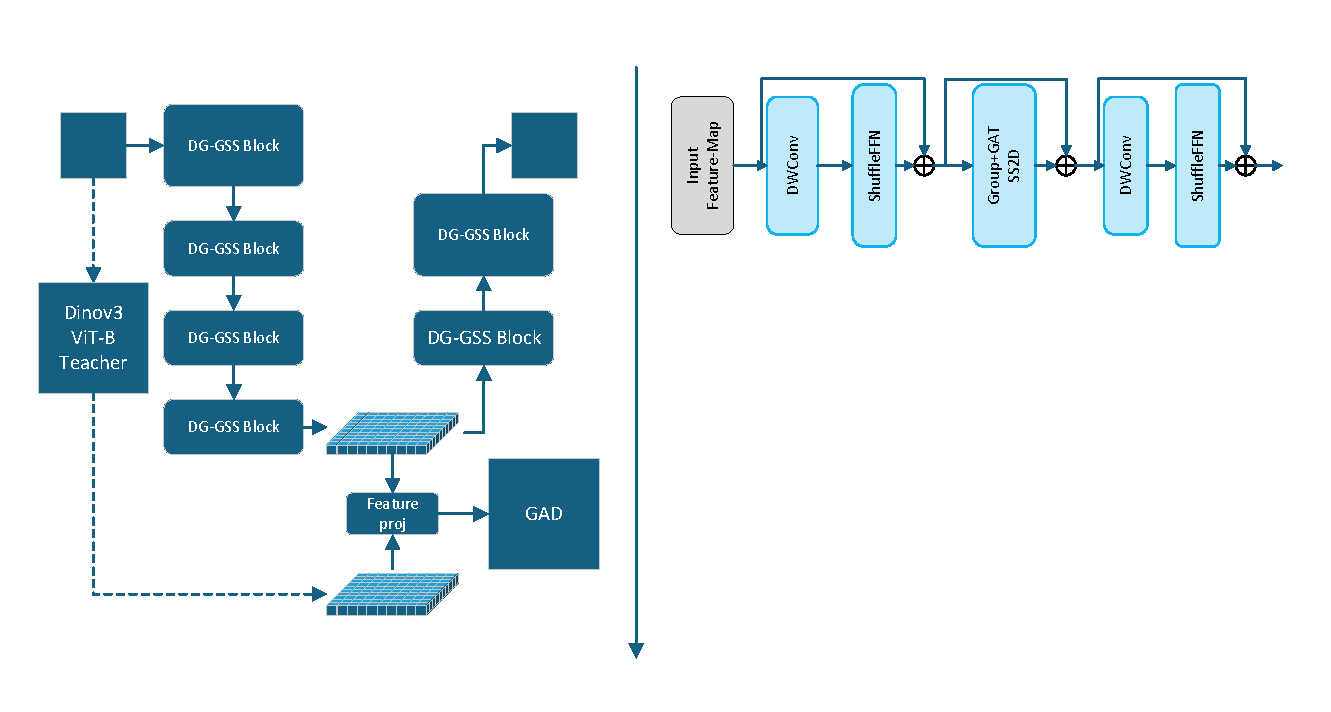
\includegraphics[width=\textwidth]{all-network.pdf}
    \caption{Overall architecture of GAD-MambaUNet. High-resolution stages retain multi-kernel local modeling, whereas deep stages use grouped state-space blocks with DG-GSS. During training, a frozen DINOv3 teacher supervises the first decoder block and GAD regulates the distillation coefficient according to its gradient share. The teacher and projection head are removed at inference.}
    \label{fig:overall-network}
\end{figure*}

\section{Methodology}


We describe the proposed GAD-MambaUNet by first introducing its core building block and then integrating it into an asymmetric U-shaped segmentation architecture. 
As shown in Fig.~\ref{fig:overall-network}, the left part presents the overall student network and the training-time DINOv3 teacher, while the right part details the proposed block-level design and the internal structure of Direction-Group Graph Selective Scan (DG-GSS). 
We first present DG-GSS, which enables structured interaction among scan directions and channel groups. Then, we describe how DG-GSS is embedded into the overall GAD-MambaUNet architecture. Finally, we introduce the training-time DINOv3 supervision with Gradient-Adaptive Distillation (GAD), where the teacher model is used only during training and removed during inference.


\subsection{Direction-Group Graph Selective Scan}

As illustrated in the lower-right part of Fig.~\ref{fig:overall-network}, DG-GSS is designed to enhance grouped multi-directional selective scanning by introducing graph-based interaction among direction--group responses. Grouped multi-directional selective scanning reduces the cost of Vision Mamba by dividing feature channels into multiple groups and processing them along several traversal directions. However, in conventional grouped scanning, each direction--group branch is processed independently and fused only after selective scanning. This independent processing limits the exchange of complementary information across scan directions and channel subspaces. To address this issue, DG-GSS regards each scan-direction and channel-group response as a graph node and performs structured message passing before the final multi-directional fusion.

Let $\mathbf{X}\in\mathbb{R}^{B\times D_i\times h\times w}$ denote the inner state-space feature of DG-GSS, where $D_i$ is the inner channel dimension. We adopt four Cross2D traversal directions and partition the inner channels into $M$ groups. With $d=D_i/M$ and $L=hw$, cross scanning produces
\begin{equation}
\mathbf{X}_{\mathrm{scan}}\in\mathbb{R}^{B\times K\times M\times d\times L},\qquad K=4.
\end{equation}

For each direction--group pair, the selective-scan parameters $(\Delta,\mathbf{B},\mathbf{C})$ are generated by independent grouped projections, and selective scanning is applied along the corresponding sequence. The directional outputs are then realigned to the original spatial coordinate system:
\begin{equation}
\mathbf{Y}\in\mathbb{R}^{B\times K\times M\times d\times h\times w}.
\end{equation}

Each tensor $\mathbf{Y}_{k,m}$ corresponds to the response of scan direction $k$ and channel group $m$. We regard every direction--group response as a graph node and obtain its node descriptor by global average pooling:
\begin{equation}
\mathbf{r}_{k,m}
=
\frac{1}{hw}
\sum_{u=1}^{h}
\sum_{v=1}^{w}
\mathbf{Y}_{k,m,:,u,v}.
\end{equation}
After layer normalization and linear projection, the node descriptor is transformed into $\mathbf{h}_{k,m}$.

In our implementation, we adopt a factorized direction-group graph, where two nodes are connected if they share the same scan direction or the same channel group, and self-connections are included. For two connected nodes $i$ and $j$, additive graph-attention logits~\cite{velickovic2018gat} are computed as
\begin{equation}
e_{ij}
=
\operatorname{LeakyReLU}
\left(
\mathbf{a}_{s}^{\top}\mathbf{h}_{i}
+
\mathbf{a}_{t}^{\top}\mathbf{h}_{j}
\right).
\end{equation}
The attention coefficients are obtained by masked softmax over the neighborhood:
\begin{equation}
\alpha_{ij}
=
\frac{\exp(e_{ij})}
{\sum_{j'\in\mathcal{N}(i)}\exp(e_{ij'})},
\qquad j\in\mathcal{N}(i).
\end{equation}

Graph-based message passing is then performed on the full spatial feature maps:
\begin{equation}
\widetilde{\mathbf{Y}}_i
=
\mathbf{Y}_i
+
\gamma
\sum_{j\in\mathcal{N}(i)}
\alpha_{ij}V(\mathbf{Y}_j),
\end{equation}
where $V(\cdot)$ is a shared $1\times1$ value projection and $\gamma$ is a learnable scaling parameter initialized to zero. This initialization makes DG-GSS start from the original grouped selective-scan behavior and progressively learn direction--group information exchange during training.

Finally, the enhanced group responses are concatenated along the channel dimension for each direction, and the four aligned directional feature maps are summed:
\begin{equation}
\mathbf{Z}
=
\sum_{k=1}^{K}
\operatorname{Concat}_{m=1}^{M}
\left(
\widetilde{\mathbf{Y}}_{k,m}
\right).
\end{equation}
Output normalization is then applied to obtain the DG-GSS output.
In this way, DG-GSS preserves the efficiency of grouped multi-directional selective scanning while explicitly modeling the structural relationship between scan directions and channel groups.



\subsection{GAD-MambaUNet Architecture}

After defining DG-GSS, we embed it into a lightweight block and integrate the block into an asymmetric U-shaped segmentation network. As shown in the upper-right part of Fig.~\ref{fig:overall-network}, the DG-GSS block consists of three residual components: a pre-scan local mixing stage, the proposed DG-GSS layer, and a post-scan local refinement stage. Given an input feature $\mathbf{x}$, the block is formulated as
\begin{equation}
\begin{aligned}
\mathbf{u}_1 &= \mathbf{x}+\operatorname{FFN}_0(\operatorname{DW}_0(\mathbf{x})), \\
\mathbf{u}_2 &= \mathbf{u}_1+\operatorname{DG\text{-}GSS}(\mathbf{u}_1), \\
\mathbf{y} &= \mathbf{u}_2+\operatorname{FFN}_1(\operatorname{DW}_1(\mathbf{u}_2)),
\end{aligned}
\end{equation}
where $\operatorname{DW}(\cdot)$ denotes depth-wise convolution for local mixing and $\operatorname{FFN}(\cdot)$ denotes a lightweight feed-forward refinement module. The local operators enhance short-range texture and channel interactions, while DG-GSS provides efficient long-range context aggregation through direction--group graph interaction.

The overall GAD-MambaUNet follows a five-level encoder--decoder architecture, as shown in the left part of Fig.~\ref{fig:overall-network}. Given an input image $\mathbf{x}\in\mathbb{R}^{3\times H\times W}$, the network predicts a binary segmentation logit map $\mathbf{z}\in\mathbb{R}^{1\times H\times W}$. In the base configuration, the channel widths are set to $[16,32,64,96,160]$. To balance local boundary preservation and global context modeling, the first three encoder stages and the last three decoder stages use lightweight multi-kernel inverted residual (MKIR) blocks inherited from MK-UNet~\cite{rahman2025mkunet}, while the two deepest encoder stages and the first two decoder stages use DG-GSS blocks. Resolution and channel changes are performed outside these blocks through depth-wise downsampling with point-wise projection or point-wise projection followed by bilinear upsampling, keeping the feature width fixed inside each block.

For decoder reconstruction, skip connections transfer high-resolution encoder features to the corresponding decoder stages. Before fusion, a grouped attention gate filters the skip feature according to the decoder context, reducing irrelevant background responses. Let $\mathbf{g}$ denote the upsampled decoder feature and $\mathbf{s}$ the encoder feature at the same resolution. The gated skip feature is computed as
\begin{equation}
\boldsymbol{\alpha}=\sigma!\left(\psi!\left(\phi(W_g\mathbf{g}+W_s\mathbf{s})\right)\right),\qquad
\hat{\mathbf{s}}=\boldsymbol{\alpha}\odot\mathbf{s},
\end{equation}
where $W_g$ and $W_s$ are grouped convolutions, $\phi$ is ReLU, and $\psi$ maps the joint response to a spatial gate. The filtered skip feature $\hat{\mathbf{s}}$ is then fused with the decoder feature. The first decoder block operates at the deepest decoder level and provides the aligned student feature for the training-time DINOv3 supervision described in the next subsection.



\subsection{Training-Time DINOv3 Supervision with GAD}

Although DG-GSS improves contextual modeling inside the compact student network, training a lightweight segmentation model on limited medical datasets may still lead to insufficient semantic abstraction. Inspired by the DINOv3-based gradient-adaptive distillation strategy in RT-DETRv4~\cite{liao2025rtdetrv4}, we adapt training-time foundation-model supervision to lightweight medical image segmentation. A frozen DINOv3 ViT-B/16 model~\cite{simeoni2025dinov3} is used as the semantic teacher only during training, and the teacher branch is removed during inference.

As described in the previous subsection, the student feature used for distillation is extracted after the first decoder block and before the first upsampling operation. This feature is semantically rich, spatially compact, and computationally inexpensive for feature alignment. Let $\mathbf{F}_{s}$ denote the projected student feature, and let $\mathbf{F}_{t}$ denote the corresponding DINOv3 teacher feature. The student feature is projected to the teacher dimension by a $1\times1$ convolution followed by batch normalization when their channel dimensions are different. If necessary, the teacher feature is bilinearly resized to match the spatial resolution of $\mathbf{F}_{s}$.

After spatial alignment, both feature maps are flattened into $N$ spatial tokens and $\ell_2$-normalized along the channel dimension. We use a cosine feature distillation loss:
\begin{equation}
\mathcal{L}_{\mathrm{dist}}
=
\frac{1}{N}\sum_{n=1}^{N}
\left[
1-
\frac{
\mathbf{f}_{s,n}^{\top}\mathbf{f}_{t,n}
}{
\left\|\mathbf{f}_{s,n}\right\|_2
\left\|\mathbf{f}_{t,n}\right\|_2
+\epsilon
}
\right],
\end{equation}
where $\mathbf{f}_{s,n}$ and $\mathbf{f}_{t,n}$ denote the $n$-th student and teacher tokens, respectively, and $\epsilon$ is a small constant for numerical stability.

The segmentation objective follows the structure-aware weighted BCE and weighted IoU loss~\cite{fan2020pranet}:
\begin{equation}
\mathcal{L}_{\mathrm{seg}}
=
\mathcal{L}_{\mathrm{wbce}}
+
\mathcal{L}_{\mathrm{wiou}}.
\end{equation}
The overall training objective is
\begin{equation}
\mathcal{L}
=
\mathcal{L}_{\mathrm{seg}}
+
\lambda_e\mathcal{L}_{\mathrm{dist}},
\end{equation}
where $\lambda_e$ is the distillation coefficient at epoch $e$.

Using a fixed distillation coefficient assumes that the proper teacher supervision strength remains unchanged throughout training. However, the optimization state of the student changes over time, and the gradient contribution of the teacher-supervised decoder block may become either too weak or too dominant. To balance semantic supervision and the primary segmentation objective, GAD dynamically updates $\lambda_e$ according to the gradient share of the aligned decoder block. After back-propagation and before gradient clipping, we compute
\begin{equation}
q_e
=
100\times
\frac{
\sum_{\theta_i\in\Theta_a}
\left\|\nabla_{\theta_i}\mathcal{L}\right\|_1
}{
\sum_{\theta_j\in\Theta}
\left\|\nabla_{\theta_j}\mathcal{L}\right\|_1
+\epsilon
},
\end{equation}
where $\Theta_a$ denotes the parameters of the aligned decoder block and $\Theta$ denotes all trainable student parameters.

Given a target gradient-share interval $[\rho-\delta,\rho+\delta]$, GAD adjusts the next-epoch distillation coefficient only when $q_e$ falls outside this interval. Let $q^{*}$ be the nearest target boundary, and define $p_e=q_e/100$ and $p^{*}=q^{*}/100$. The odds-ratio adjustment is computed as
\begin{equation}
r_e
=
\frac{
p^{*}(1-p_e)
}{
p_e(1-p^{*})+\epsilon
}.
\end{equation}
The distillation coefficient for the next epoch is updated by
\begin{equation}
\lambda_{e+1}
=
\operatorname{clip}
\left(
\lambda_e
\operatorname{clip}(r_e,r_{\min},r_{\max}),
\lambda_{\min},
\lambda_{\max}
\right),
\end{equation}
where $r_{\min}$ and $r_{\max}$ bound the per-epoch adjustment, and $\lambda_{\min}$ and $\lambda_{\max}$ constrain the overall distillation strength.

Training begins with a segmentation-only burn-in stage, followed by a linear distillation warm-up. GAD is activated after warm-up to adaptively regulate the teacher contribution. During inference, the DINOv3 teacher, the feature projection head, and the GAD update are all discarded. Therefore, the proposed training-time supervision improves the compact student without increasing deployment cost.


% \section{Methodology}

% \subsection{Overview}

% Fig.~\ref{fig:overall-network} presents GAD-MambaUNet. Given an image $\mathbf{x}\in\mathbb{R}^{3\times H\times W}$, the student produces a binary logit map $\mathbf{z}\in\mathbb{R}^{1\times H\times W}$. The base model uses five resolution levels with channel widths $[16,32,64,96,160]$. The first three encoder blocks and the last three decoder blocks are multi-kernel inverted residual (MKIR) blocks. The two deepest encoder blocks and the first two decoder blocks are grouped Mamba blocks. Resolution and channel changes are performed outside these blocks by depth-wise downsampling followed by point-wise projection, or by point-wise projection followed by bilinear upsampling. This separation keeps the state-space width fixed within each block.

% At every decoder level, channel and spatial attention refine the decoder feature, while a grouped attention gate filters the corresponding skip connection before additive fusion. The first decoder block operates at $H/32\times W/32$ and supplies the student feature used for DINOv3 supervision. This location is semantically rich, inexpensive, and directly aligned with the block monitored by GAD.

% \subsection{Asymmetric Local--Global Student}

% At high resolution, the dominant requirement is local boundary reconstruction. We therefore retain the MKIR design of MK-UNet~\cite{rahman2025mkunet}: a $1\times1$ expansion, parallel depth-wise convolutions with kernels $\mathcal{K}=\{1,3,5\}$, summation, channel shuffle, and a $1\times1$ projection. For feature $\mathbf{x}$, the block is written compactly as
% \begin{equation}
% \operatorname{MKIR}(\mathbf{x})=
% P_2\!\left(\operatorname{Shuffle}\!\left[
% \sum_{k\in\mathcal{K}}D_k\!\left(P_1(\mathbf{x})\right)\right]\right),
% \end{equation}
% where $P_1$ and $P_2$ denote point-wise expansion and projection and $D_k$ is a depth-wise convolution with kernel size $k$. The block supplies multi-receptive-field local evidence at low cost.

% At low resolution, the receptive field can be enlarged more efficiently. A grouped Mamba block first applies depth-wise local mixing and a grouped shuffle feed-forward network (FFN), then DG-GSS, and finally a second local mixing--FFN pair. Each component is residual:
% \begin{equation}
% \begin{aligned}
% \mathbf{u}_1 &= \mathbf{x}+\operatorname{FFN}_0(\operatorname{DW}_0(\mathbf{x})),\\
% \mathbf{u}_2 &= \mathbf{u}_1+\operatorname{DG\text{-}GSS}(\mathbf{u}_1),\\
% \mathbf{y} &= \mathbf{u}_2+\operatorname{FFN}_1(\operatorname{DW}_1(\mathbf{u}_2)).
% \end{aligned}
% \end{equation}
% The local operators therefore refine state-space features instead of competing with them.

% For skip fusion, let $\mathbf{g}$ denote the upsampled decoder feature and $\mathbf{s}$ the encoder feature at the same resolution. A grouped attention gate computes
% \begin{equation}
% \boldsymbol{\alpha}=\sigma\!\left(\psi\!\left(\phi(W_g\mathbf{g}+W_s\mathbf{s})\right)\right),\qquad
% \hat{\mathbf{s}}=\boldsymbol{\alpha}\odot\mathbf{s},
% \end{equation}
% where $W_g$ and $W_s$ are grouped convolutions, $\phi$ is ReLU, and $\psi$ maps the joint response to a spatial gate. The decoder feature and $\hat{\mathbf{s}}$ are then added.

% \subsection{Direction-Group Graph Selective Scan}

% Let $\mathbf{X}\in\mathbb{R}^{B\times D\times h\times w}$ be the input to DG-GSS. We use four Cross2D traversal directions and partition the inner state-space channels into $M$ groups. With $d=D/M$ and $L=hw$, cross scanning yields
% \begin{equation}
% \mathbf{X}_{\mathrm{scan}}\in\mathbb{R}^{B\times K\times M\times d\times L},\qquad K=4.
% \end{equation}
% Every direction--group pair independently produces its selective-scan parameters $(\Delta,\mathbf{B},\mathbf{C})$. Selective scan is applied to each pair and the four outputs are spatially realigned to the original coordinate system:
% \begin{equation}
% \mathbf{Y}\in\mathbb{R}^{B\times K\times M\times d\times h\times w}.
% \end{equation}

% The tensor $\mathbf{Y}_{k,m}$ is a response from direction $k$ and channel group $m$. We regard it as a graph node and obtain a node descriptor by global average pooling:
% \begin{equation}
% \mathbf{r}_{k,m}=\frac{1}{hw}\sum_{u,v}\mathbf{Y}_{k,m,:,u,v}.
% \end{equation}
% After layer normalization and linear projection, additive graph-attention logits~\cite{velickovic2018gat} are
% \begin{equation}
% e_{ij}=\operatorname{LeakyReLU}\left(\mathbf{a}_{s}^{\top}\mathbf{h}_i+
% \mathbf{a}_{t}^{\top}\mathbf{h}_j\right).
% \end{equation}
% Our factorized adjacency connects two nodes when they have the same scan direction or the same channel-group identity, including self-connections. Thus, a node receives both cross-group and cross-direction evidence without constructing an unconstrained fully connected graph. With masked softmax weights $a_{ij}$ and shared $1\times1$ value projection $V(\cdot)$, graph propagation is
% \begin{equation}
% \widetilde{\mathbf{Y}}_i=\mathbf{Y}_i+\gamma\sum_{j\in\mathcal{N}(i)}a_{ij}V(\mathbf{Y}_j),
% \end{equation}
% where $\gamma$ is learnable and initialized to zero. DG-GSS consequently starts from the original grouped scan behavior and learns graph exchange progressively. Finally, groups are concatenated and the four aligned directions are summed before output normalization.

% \subsection{DINOv3 Supervision and Gradient-Adaptive Distillation}

% A frozen DINOv3 ViT-B/16 teacher provides dense features only during training. The feature $\mathbf{F}_s$ after the first decoder block is projected by a $1\times1$ convolution and batch normalization to the teacher dimension. The teacher feature $\mathbf{F}_t$ is bilinearly resized when necessary. After flattening each map into spatial tokens and applying $\ell_2$ normalization, the feature loss is
% \begin{equation}
% \mathcal{L}_{\mathrm{dist}}=
% \frac{1}{N}\sum_{n=1}^{N}\left[1-
% \frac{\mathbf{f}_{s,n}^{\top}\mathbf{f}_{t,n}}
% {\|\mathbf{f}_{s,n}\|_2\|\mathbf{f}_{t,n}\|_2}\right].
% \end{equation}
% The segmentation objective follows the structure-aware weighted BCE and weighted IoU loss~\cite{fan2020pranet}:
% \begin{equation}
% \mathcal{L}=\mathcal{L}_{\mathrm{seg}}+\lambda_e\mathcal{L}_{\mathrm{dist}},
% \qquad
% \mathcal{L}_{\mathrm{seg}}=\mathcal{L}_{\mathrm{wbce}}+\mathcal{L}_{\mathrm{wiou}}.
% \end{equation}

% Using a fixed $\lambda_e$ assumes that the appropriate teacher pressure remains unchanged throughout training. Instead, after backpropagation and before gradient clipping, GAD measures the gradient share of the aligned decoder block:
% \begin{equation}
% q_e=100\times
% \frac{\sum_{\theta_i\in\Theta_a}\|\nabla_{\theta_i}\mathcal{L}\|_1}
% {\sum_{\theta_j\in\Theta}\|\nabla_{\theta_j}\mathcal{L}\|_1}.
% \end{equation}
% Here, $\Theta_a$ is the parameter set of decoder1 and $\Theta$ contains all student parameters. If $q_e$ falls outside the target interval $[\rho-\delta,\rho+\delta]$, GAD selects the opposite interval boundary as $q^*$ and computes an odds-ratio adjustment:
% \begin{equation}
% r_e=\frac{p^{*}(1-p_e)}{p_e(1-p^{*})},
% \quad p_e=q_e/100,\quad p^{*}=q^{*}/100.
% \end{equation}
% The next base distillation coefficient is
% \begin{equation}
% \lambda_{e+1}=\operatorname{clip}\left(
% \lambda_e\operatorname{clip}(r_e,r_{\min},r_{\max}),
% \lambda_{\min},\lambda_{\max}\right).
% \end{equation}
% The multiplicative adjustment is bounded per epoch and the coefficient is clipped to $[\lambda_{\min},\lambda_{\max}]$ for stability. Training begins with segmentation-only burn-in, follows with a linear distillation warm-up, and activates GAD after warm-up. At inference, the teacher, feature projection head, and GAD update are discarded.


\section{Experiments and Results}
\label{sec:experiments}

\subsection{Datasets and Metrics}

We evaluate GAD-MambaUNet on four public binary medical image segmentation datasets covering two representative segmentation tasks. For skin lesion segmentation, we use PH$^2$~\cite{mendoncca2013ph}, which contains 200 dermoscopic images with expert lesion annotations, and ISIC2018~\cite{codella2019skin}, which contains 2,594 dermoscopic images with pixel-level lesion masks. For polyp segmentation, we use CVC-ClinicDB~\cite{bernal2015clinicdb}, which contains 612 colonoscopic polyp images, and CVC-ColonDB~\cite{tajbakhsh2016colondb,vazquez2017benchmark}, which contains 379 colonoscopic images collected from different video sequences. These datasets include diverse imaging conditions, lesion appearances, object scales, boundary ambiguities, and foreground--background contrasts, providing a comprehensive evaluation of the robustness of lightweight segmentation models.

We split each dataset into training, validation, and test subsets with a ratio of 80:10:10. The validation set is used for model selection, and the test set is used for final performance reporting. Dice score is used as the primary segmentation metric, and Intersection over Union (IoU) is also reported when applicable. To evaluate model efficiency, we report the number of trainable parameters and floating-point operations (FLOPs). Since the DINOv3 teacher is used only during training and is discarded during deployment, it does not introduce additional inference computation. Therefore, all efficiency metrics are computed using the student network alone.

\subsection{Implementation Protocol}


All experiments are implemented in PyTorch and conducted under the same training and evaluation settings for fair comparison. Images from PH$^2$ and ISIC2018 are resized to $256\times256$, while images from CVC-ClinicDB and CVC-ColonDB are resized to $352\times352$. The validation set is used for checkpoint selection, and the corresponding test performance is reported.

For GAD-MambaUNet, we use AdamW as the optimizer with an initial learning rate of $5\times10^{-4}$, a weight decay of $10^{-4}$, and cosine learning-rate decay to $10^{-6}$. All models are trained for 400 epochs with a batch size of 8, gradient clipping at 0.5, and standard data augmentation. The segmentation objective is the sum of weighted binary cross-entropy and weighted IoU losses. Unless otherwise specified, each configuration is repeated over five independent runs, and the mean test performance is reported.

For training-time semantic supervision, we use frozen DINOv3 ViT-T/16 and ViT-B/16 models as semantic teachers in different experimental settings. The student feature after the first decoder block is aligned to the teacher feature through the projection head described in Section~\ref{sec:method}. DINOv3 distillation starts at epoch 10 and is linearly warmed up for 20 epochs. GAD is activated at epoch 30 and adaptively controls the distillation coefficient until epoch 360. During inference, the teacher branch, projection head, and GAD update are discarded, so the reported parameters and FLOPs are computed using only the student network.

\begin{table*}[t]
    \centering
    \caption{Comparison on four datasets. Non-PH$^2$ baseline values are taken from the original MK-UNet paper under its reported protocol. Dice scores are reported in \%. PH$^2$, ClinicDB, and ColonDB entries for MK-UNet and GAD-MambaUNet are mean test Dice at the validation-selected checkpoint over repeated runs. DINOv3 is used only during training and adds no inference cost.}
    \label{tab:reference_results}
    \scriptsize
    \resizebox{\textwidth}{!}{%
    \begin{tabular}{lcccccccc}
        \toprule
        Method & Params(M) & FLOPs(G) & Throughput(/s) & PH$^2$ & ISIC2018 & ClinicDB & ColonDB & Avg. \\
        \midrule
        U-Net & 34.53 & 65.53 & 119.03 & -- & 86.67 & 91.43 & 83.95 & -- \\
        PraNet & 32.55 & 6.93 & 64.10 & -- & 88.46 & 91.71 & 89.16 & -- \\
        UACANet & 69.16 & 31.51 & 43.28 & -- & 88.72 & 93.29 & 89.76 & -- \\
        TransUNet & 105.32 & 38.52 & 65.35 & -- & 89.04 & 93.18 & 89.97 & -- \\
        UNeXt & 1.47 & 0.57 & 172.41 & -- & 87.78 & 90.20 & 83.84 & -- \\
        CMUNeXt & 0.418 & 1.09 & 175.43 & -- & 87.51 & 92.82 & 83.85 & -- \\
        EGE-UNet & 0.054 & 0.072 & 101.01 & -- & 86.95 & 84.76 & 76.03 & -- \\
        UltraLight VM-UNet & 0.050 & 0.060 & 98.03 & -- & 87.85 & 87.11 & 80.06 & -- \\
        MK-UNet-T & 0.027 & 0.062 & 140.85 & 94.56 & 88.19 & 91.26 & 85.03 & -- \\
        MK-UNet & 0.316 & 0.314 & 138.89 & 94.39 & 88.74 & 93.48 & 90.01 & -- \\
        MK-UNet-L & 3.76 & 3.19 & 122.62 & 94.56 & 89.25 & 93.85 & 91.82 & -- \\
        \midrule
        GAD-MambaUNet-Tiny (Ours) & 0.076 & 0.051 & -- & 94.43 & 88.27 & 92.47 & 83.20 & -- \\
        GAD-MambaUNet-Small (Ours) & 0.199 & 0.117 & -- & 94.40 & 88.63 & 93.85 & 90.17 & -- \\
        GAD-MambaUNet-Base (Ours) & 0.493 & 0.291 & -- & \textbf{94.90} & 88.91 & 94.04 & 91.24 & -- \\
        GAD-MambaUNet-Medium (Ours) & 1.839 & 0.955 & -- & 94.71 & 89.13 & 94.07 & 91.35 & -- \\
        GAD-MambaUNet-Large (Ours) & 5.871 & 3.325 & -- & 94.88 & 89.34 & \textbf{94.70} & \textbf{92.16} & -- \\
        \midrule
        GAD-MambaUNet-Tiny + DINOv3 (Ours) & 0.076 & 0.051 & -- & 94.61 & 88.61 & 93.09 & 86.54 & -- \\
        GAD-MambaUNet-Small + DINOv3 (Ours) & 0.199 & 0.117 & -- & 94.73 & 88.94 & 94.16 & 91.51 & -- \\
        GAD-MambaUNet-Base + DINOv3 (Ours) & 0.493 & 0.291 & -- & 95.16 & 89.06 & 94.17 & 91.96 & -- \\
        GAD-MambaUNet-Medium + DINOv3 (Ours) & 1.839 & 0.955 & -- & 95.21 & 89.11 & 94.52 & \textbf{93.08} & -- \\
        GAD-MambaUNet-Large + DINOv3 (Ours) & 5.871 & 3.325 & -- & 95.37 & 89.53 & 95.08 & 93.01 & -- \\
        \bottomrule
    \end{tabular}
    }
\end{table*}

\subsection{Reference Baseline Analysis}

Table~\ref{tab:reference_results} summarizes the reference landscape together with the completed CVC-ClinicDB and CVC-ColonDB scaling runs of GAD-MambaUNet. Fig.~\ref{fig:efficiency-comparison} further visualizes the average Dice--efficiency trade-off against student-side parameters and FLOPs. Heavy encoder-decoder and Transformer-based models, such as TransUNet, provide strong Dice scores but require substantially more parameters and computation. Lightweight CNN and state-space models reduce the computational footprint, but their performance varies across modalities: some are effective on skin lesions but degrade on colonoscopic polyp datasets where boundary ambiguity and background similarity are more severe.

MK-UNet provides a strong local-convolutional baseline with a compact parameter count and competitive Dice scores across the four datasets. This makes it an appropriate reference point for our design. Without DINOv3 supervision, performance rises sharply from Tiny to Base and then largely saturates, with Large achieving the highest validation-selected ColonDB test Dice. Adding DINOv3 supervision improves the Medium variant to the best reported ColonDB score, while retaining the same student-side inference cost. The remaining experiments will determine whether GAD further improves this trade-off.

\section{Ablation Study}
\label{sec:ablation}

The ablation study is designed to separate the contribution of the three main design choices: deep grouped state-space modeling, direction-group graph interaction, and gradient-adaptive DINOv3 distillation. Table~\ref{tab:ablation_plan} lists the planned variants. All variants will use the same data split, preprocessing, segmentation loss, and training schedule, so the measured differences can be attributed to architectural and distillation changes.

\begin{table}[t]
    \centering
    \caption{Planned ablation variants for GAD-MambaUNet. Values are left blank until the corresponding experiments are completed.}
    \label{tab:ablation_plan}
    \scriptsize
    \resizebox{\columnwidth}{!}{%
    \begin{tabular}{lccccc}
        \toprule
        Variant & BUSI & ISIC2018 & ClinicDB & ColonDB & Avg. \\
        \midrule
        Local student baseline & -- & -- & -- & -- & -- \\
        + Grouped Mamba blocks & -- & -- & -- & -- & -- \\
        + DG-GSS & -- & -- & -- & -- & -- \\
        + DINOv3 fixed distillation & -- & -- & -- & -- & -- \\
        + GAD distillation & -- & -- & -- & -- & -- \\
        \bottomrule
    \end{tabular}
    }
\end{table}

\subsection{Effect of Direction-Group Global Modeling}

The first ablation compares the local student baseline with variants that insert grouped Mamba blocks and DG-GSS into the deep encoder-decoder stages. This comparison tests whether global context is beneficial when introduced only at low spatial resolutions. A positive result would indicate that long-range dependencies can be added without disturbing the high-resolution local features used for boundary reconstruction.

\subsection{Effect of DINOv3 Distillation}

The second ablation compares training without distillation, training with a fixed DINOv3 distillation coefficient, and training with GAD. Fixed distillation measures whether dense foundation-model features provide useful semantic regularization. GAD further measures whether adapting the teacher weight according to the student's gradient distribution stabilizes the transfer and improves the final mask quality.

\section{Conclusion}
\label{sec:conclusion}

This paper presents GAD-MambaUNet, a lightweight medical image segmentation framework that combines high-resolution multi-kernel local modeling, deep direction-group state-space interaction, and gradient-adaptive DINOv3 feature distillation. The design keeps inference compact by using the foundation model only during training, while targeting the common failure modes of binary medical segmentation: weak boundaries, appearance ambiguity, and insufficient global context. Initial CVC-ClinicDB and CVC-ColonDB scaling results without DINOv3 show that strong accuracy is attainable with sub-megaparameter variants, while Large gives the strongest reported validation-selected ColonDB result. The remaining multi-dataset and distillation ablations will complete the evaluation.

\bibliographystyle{IEEEtran}
\bibliography{paper_refs}

\end{document}
